\begin{ledgroupsized}[r]{120mm}
\footnotesize 
\pstart    
\noindent\textbf{\"{U}berlieferung:} 
\pend
\end{ledgroupsized}
\begin{ledgroupsized}[r]{114mm}
\footnotesize 
\pstart \parindent -6mm
\makebox[6mm][l]{\textit{L}}%
Reinschrift mit Verbesserungen: LH XXXV 10, 9 Bl. 1. 1 Bl. 4\textsuperscript{o}. 1 S. auf Bl.~1~r\textsuperscript{o}. Bl.~1~v\textsuperscript{o} leer. Unvollständige Abschrift von N. 28\textsubscript{2}.
\\ 
Cc 2, Nr. 1190 A
\pend
\end{ledgroupsized}
\count\Bfootins=1200
\vspace*{8mm}
%\pstart 
%\normalsize
%{\centering[1~r\textsuperscript{o}] Regle\\
%pour calculer la force\protect\index{Sachverzeichnis}{force} d'une\\
%Machine\protect\index{Sachverzeichnis}{machine}, dont voicy la figure\\}
\pstart 
\normalsize
\noindent
[1~r\textsuperscript{o}]
\pend
\pstart
\centering
\noindent
Regle pour calculer la force d'une Machine,\protect\index{Sachverzeichnis}{machine}\protect\index{Sachverzeichnis}{force}\\%
dont voicy la figure
\pend
\vspace{1.0em}
\pstart
\noindent
Soit la roue\protect\index{Sachverzeichnis}{roue} \textit{ABCD} mobile \`{a} l'entour du \edtext{centre \textit{L},}{\lemma{centre \textit{L}}\Bfootnote{\textit{(1)} . Supposons qu'elle est \textit{(2)} , entrecoup\'{e}e \textit{L}\hspace{-2mm}}} \edtext{entrecoup\'{e}e \`{a} angles \mbox{droits} de deux}{\lemma{}\Bfootnote{\`{a} angles droits \textit{erg. L}\hspace{-2mm}}} Diametres\protect\index{Sachverzeichnis}{diametre} solides \textit{AC}, et \textit{DB}; les quels seront transferez par le mouuement\protect\index{Sachverzeichnis}{mouvement} \`{a} l'entour du centre, de la situation perpendiculaire ou \edtext{horizontale, \mbox{\textit{ABCD}}, \`{a} l'inclin\'{e}e}{\lemma{}\Bfootnote{\textit{ABCD}, \textit{erg. L}}} \textit{EFGH} dans un \textso{angle donn\'{e}} \textit{ALE}. Conceuuons la dite roue charg\'{e}e dans les points, \textit{E}, \textit{F}, \textit{K}, \textit{I}, de quatre poids \'{e}gaux entre eux.
\pend
\vspace{1.5em}
\pstart
\centering
%\begin{wrapfigure}[17]{l}{0.5\textwidth}
%\vspace{-4mm}
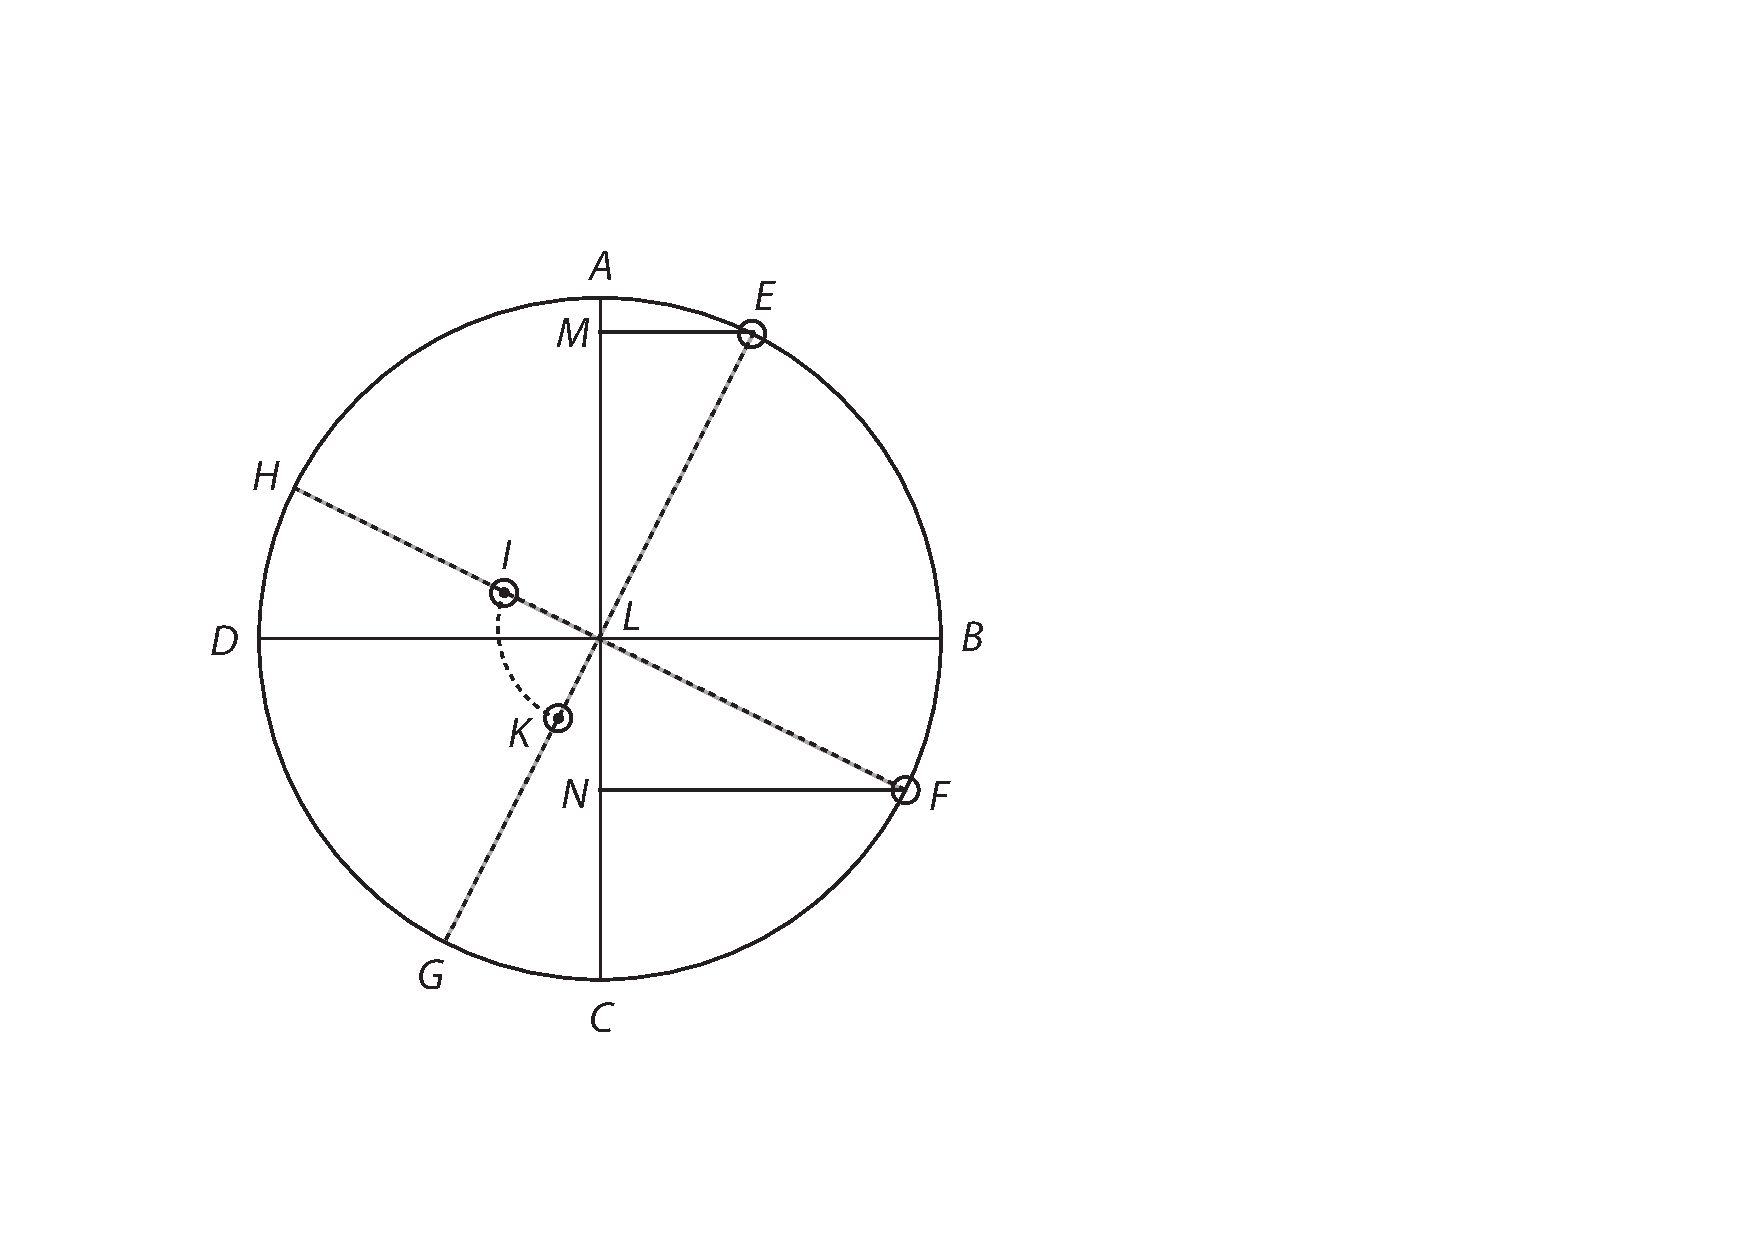
\includegraphics[trim = 0mm 0mm 0mm 0mm, clip, width=0.5\textwidth]{images/lh0351009_001r-d1.pdf}\\
\noindent \centering [\textit{Fig. 1}]
%\caption{Bildbeschreibung}
%\end{wrapfigure}
\pend
\newpage
\pstart
\indent Soit \textso{donn\'{e}e} la longueur de \textit{AC}, diametre\protect\index{Sachverzeichnis}{diametre} de la Roue, item la longueur des droites \textit{ELK}, ou \textit{FLI} \'{e}gales entre elles.\\
\indent Et enfin \textso{la force absolue}\protect\index{Sachverzeichnis}{force absolue} d'un de ces poids, c'est \`{a} dire avec la quelle il agit libr\`{e}ment, ou sur un plan parallele \`{a} l'horison, s'il en 
estoit soutenu.\\
\indent On demande la \edtext{force\protect\index{Sachverzeichnis}{force} de la machine\protect\index{Sachverzeichnis}{machine}, qu'elle auroit dans}{\lemma{force}\Bfootnote{\textit{(1)}\ absolue de la machine\protect\index{Sachverzeichnis}{machine}, dans \textit{(2)}\ de la machine\protect\index{Sachverzeichnis}{machine}, qu'elle auroit dans \textit{L}}} l'Estat \textit{EFGH}, si elle y commenceroit le mouuement\protect\index{Sachverzeichnis}{mouvement}; car il faut adjouter cette condition \`{a} fin de ne pas embarasser le calcul de la force simple\protect\index{Sachverzeichnis}{force simple}, par celuy de la force gagn\'{e}e\protect\index{Sachverzeichnis}{force gagn\'{e}e} 
par l'acceleration\protect\index{Sachverzeichnis}{acceleration}, \edtext{dont le calcul\protect\index{Sachverzeichnis}{calcul} se doit}{\lemma{dont}\Bfootnote{\textit{(1)}\ il faut \textit{(2)}\ le calcul se
doit \textit{ L}}} faire \`{a} part. 
\pend 
%\newpage
\pstart
Des points, \textit{E.F} menez les perpendiculaires \textit{EM}, \textit{FN}, sur le diametre\protect\index{Sachverzeichnis}{diametre} vertical \textit{AC}, les quelles seront \textso{donn\'{e}es}, par ce que les Angles \textit{ALE}, \textit{CLF} sont donn\'{e}s, dont elles sont les 
sinus droits. 
\pend 
\pstart
\textso{Cela estant pos\'{e}, je dis que la force absolue\protect\index{Sachverzeichnis}{force absolue} d'un des poids susdits est \`{a} la force\protect\index{Sachverzeichnis}{force} de la machine, comme le rect}\-\textso{angle \textit{ELK} (: ou compris soubs \textit{EL}, \textit{LK} :) est au rectangle compris soubs \textit{HI} et \textit{MN}.}\pend \pstart
Theoreme assez beau, et d'un tres grand usage pour le calcul des mouuements\protect\index{Sachverzeichnis}{mouvement} circulaires. \pend \pstart
Pour donner cette raison en nombres, il faut se servir des lettres de l'Analyse\protect\index{Sachverzeichnis}{analyse}, qui signifient des nombres indefinis, 
\pend 
\count\Bfootins=1500
\pstart
Soit
\begin{tabular}[t]{lr}
le sinus droit \textit{EM} appell\'{e},&\textit{y}\hspace{0.1mm}\\
le Rayon \textit{AL}&\textit{a}\\
le petit Rayon \textit{LI}&\textit{b}\\
\end{tabular}
\pend
\vspace{1mm}
\pstart\noindent
et\setline{23} la force absolue\protect\index{Sachverzeichnis}{force absolue} d'un des poids
sera \`{a} la force de la Machine\protect\index{Sachverzeichnis}{machine},
comme est 1, ou l'unit\'{e}, \`{a} $\rule[-4mm]{0mm}{12mm}\displaystyle\frac{y + \sqrt{a^2 - y^2}, \smallfrown a - b}{ba}$
ou comme 1,
\`{a} $\rule[-4mm]{0mm}{10mm}\displaystyle\frac{ya - yb + a\sqrt{a^2 - y^2} - b\sqrt{a^2 - y^2}}{ba}$. 
\pend